\chapter{引言}
\section{项目背景}
1920年我国第一条民用航线开航,一百年后飞机早已是寻常百姓家的出行选择。《2021年全国民用运输机场生产统计公报》\cite{minhang}显示,2021年我国境内民用机场已达248个,在地域广袤的中西部,机场几乎是城市标配。
同时《2022年度全球民航航班运行报告》\cite{variflight}显示,新冠疫情背景下2022年度国内航线实际执行客运航班量仍达239万架次,且相比2019年疫情前刚恢复五成以上。航空较陆路有更复杂的安全因素,民用航班的普及离不开航空安全的精进。据《国际航协2021年全球航空运输安全报告》\cite{iata}统计,2021年客机所属涡轮螺旋桨飞机每百万次飞行发生1.77起损毁,5年内平均值
为1.22。这一方面得益于成熟的飞机制造,另一方面全动飞行模拟机(Full Flight Simulator 以下简称为 FFS)为飞行员提供身临其境的训练环境功不可没。
\par
FFS是由模拟座舱、视景系统、声音系统、运动系统、网络系统和仿真机构成的飞行训练工具\cite{simulator3}。汽车驾驶员可以驾驶符合驾照类别的任意汽车,而民航飞行员想获取某型号飞机的驾驶资格,必须在对应型号FFS上进行日常训练。因此新机型若想步入市场,配套FFS不可或缺。我国航空市场广阔,且国产大飞机C919已蓄势待发,FFS需求旺盛,但目前该领域仍主要依靠行业巨擘加拿大CAE公司。
进口产品购置成本高,二次开发困难,且可能面临技术封锁。为降低成本与风险,FFS的国产化迫在眉睫。
\par
本文中基于自研游戏引擎开发的视景系统是最终实现FFS国产化的重要组成部分。
一台FFS的核心是仿真机,它相当于整个FFS的后台,负责根据飞行员在模拟座舱中的输入操作计算生成各类指令。各个系统运作均由来自仿真机的控制。视景系统负责根据仿真机指令中的位置信息从地景数据库中加载周边地形地貌,并结合时间,天气等综合信息实时渲染座舱前方的仿真景象;飞行中产生的如碰撞等异常行为也由视景系统反馈给仿真机。业界将视景系统中负责逻辑计算和渲染的该部分统称为图像生成器(Image Generator)。
由此可见开发视景系统离不开仿真机的支持,本视景系统便是基于国内占有量最高的CAE仿真机开发。
\par
经过对多种仿真机抓包分析后,发现问题在于仿真机是一个非常底层的设备,从网络模型角度看其最高层是数据链路层,指令数据用以太网协议封装后便进行发送,接收数据也只能仅被以太网协议封装过,否则无法正确解读。因此无法通过工作于传输层以上的传统socket连接模式与本视景系统中的图像生成器交流。
为了使位于不同网络体系结构层级的仿真机与图像生成器沟通,本文为视景系统设计了数据交换子系统。一方面连接仿真机,收发仅用以太网协议封装的数据帧,转换为自拟指令类型后,通过传统网络体系层层封装再与图像生成器交互。
这不仅解决了图像生成器与仿真机的交流问题,还屏蔽了不同厂商仿真机间数据组织结构的差异,保留了搭载于多种仿真机上的可能。
\par
其次在真实训练环境下,模拟座舱前方是一个球幕,需要多个图像生成器同时工作进行融合投影才能产生良好的视觉效果。但出于网络波动和TCP仅支持单播的特点,数据到达各图像生成器的时间存在差异,导致最终的融合投影产生画面撕裂。
为解决该问题,在图像生成器侧设计了网络帧缓冲机制和多种插值方法,使得多台设备逻辑线程可以做到几乎同时使用相同的数据进行计算。
\par
目前本视景系统以适配国内仍大量服役的进口仿真机为短期目标,同时也为搭载于孕育中的国产仿真机做准备,期待国产FFS能够早日走进各大飞行训练基地。
\section{国内外相关技术的发展概况}
\subsection{飞行模拟机}
世界上第一架飞机于1903年由莱特兄弟试飞成功,最初的飞行模拟机则诞生于1910年,仅具备三个维度的手动旋转功能\cite{simhis1}。 1917年,法国的Lender和Heildelbergof发明了燃油驱动旋转的版本\cite{simhis2}。而现代飞行模拟机的雏形则是发明于1930纯电气驱动的Linker Trainer,它在1937年被美国航空公司引入。
之后在二战和电子计算机的刺激下,飞行模拟机逐渐发展出更复杂体系和更真实的感官效果\cite{simulator2}。
\par
现代飞行模拟机的种类很多,从大的方面来看,基本可以分为试验用飞行模拟机和训练用飞行模拟机两大类。
试验用飞行模拟机主要用于新型飞机研制或旧机型改进。
训练用飞行模拟机早已拥有完备的标准。国际民航组织ICAO于1995年发布《飞行模拟鉴定标准手册》并持续更新\cite{normalize2},所有现代商业飞行模拟机均需要按照标准设计,通过鉴定后才可以用于飞行员培训。我国于2005年由中国民用航空总局正式颁发的CCAR-60《飞行模拟设备的鉴定和使用规则》作为
国内航空公司飞行员模拟训练设备的鉴定标准,并于2019年重新修订\cite{normalize1}。《规则》中说明我国训练用飞行模拟机分为A、B、C、D四个等级,其中D级为最高标准,即要达成《规则》文件中的全部最高标准,
才可以作为全程飞行训练的模拟机。C、B、A三个等级则是在响应时间,功能完整性方面逐步放宽要求,可以用于一些专项训练。
表\ref{viscomp}提供了《规则》中视景系统部分标准的对比。图\ref{simout}与图\ref{siminn}提供了D级模拟机外部和内部样貌。
\begin{table}[h!]
    \begin{center}
        \caption{视景系统部分标准对比}
        \label{viscomp}
        \renewcommand\arraystretch{1.2}
        \begin{tabularx}{\textwidth}{ 
            | >{\centering\arraybackslash\hsize=0.5\hsize\linewidth=\hsize}X 
            | >{\centering\arraybackslash\hsize=0.125\hsize\linewidth=\hsize}X 
            | >{\centering\arraybackslash\hsize=0.125\hsize\linewidth=\hsize}X 
            | >{\centering\arraybackslash\hsize=0.125\hsize\linewidth=\hsize}X 
            | >{\centering\arraybackslash\hsize=0.125\hsize\linewidth=\hsize}X 
            | }
            \hline
            \textbf{视景系统要求} & \textbf{A} & \textbf{B} & \textbf{C} & \textbf{D}\\
            \hline
            视景系统不应具有导致不真实特性的光学不连续性和人工痕迹。 & √ & √ & √ & √\\
            \hline
            模拟机应当在每个驾驶员座位上提供连续最小水平90°、垂直40°的准直视场。 & & & √ & √\\
            \hline
            视景系统应当提供着陆期间判断下降率(深度感觉)所必须的目视提示。 & & √ & √ & √\\
            \hline
            提供黄昏和黎明视景,保证环境光强度减弱的色彩表征。 & & & √ & √\\
            \hline
            模拟机应当能在起飞、进近和着陆期间表现雷暴附近的轻度、中度和重度降水的特殊天气。 & & & & √\\
            \hline
            模拟机应当表现全部机场灯光的真实颜色和方向性。 & & & & √\\
            \hline
        \end{tabularx}
    \end{center}
\end{table}
\begin{figure}[h!]
    \begin{minipage}[t]{0.48\textwidth}
        \centering
        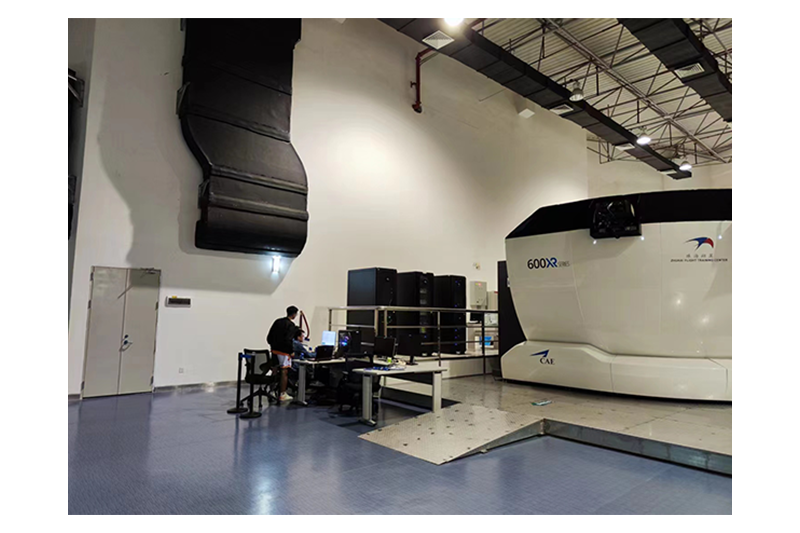
\includegraphics[width=6cm]{pictures/simulator.png}
        \caption{D级模拟机外部}
        \label{simout}
    \end{minipage}
    \begin{minipage}[t]{0.48\textwidth}
        \centering
        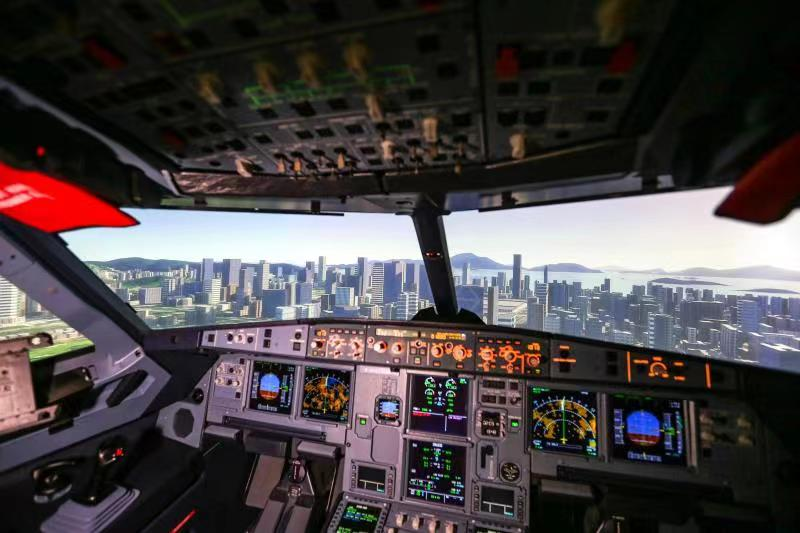
\includegraphics[width=6cm]{pictures/simulator.jpg}
        \caption{D级模拟机内部}
        \label{siminn}
    \end{minipage}
\end{figure}
\par
近年来我国用于飞行员训练的D级模拟机均来自CAE、Flight Safety等国外模拟机制造商。2020年8月,北京蓝天航空科技有限公司研发的新舟60飞机对应的全动模拟机通过了D级飞行模拟机认证,开始打破国外模拟机制造商对于D级飞行模拟机研制的垄断,迈出了国产模拟机的坚实一步\cite{simhis3}。
但新舟60本已是几近停飞的老旧型号飞机,市场存量很小,更复杂的市场主流型号客机以及C919客机模拟机的自主研发仍在进程中。
\subsection{视景系统}
最早的飞行模拟机并不具备视景系统,驾驶员仅能在地面上体验旋转。在上世纪30年代,一个位于机身前循环播放的画轴被视为第一个视景系统。60年代闭路电视的发展让视景系统有了新形态,让相机扫过带有场景的皮带再将画面投影至飞行员眼前\cite{vishis1},此设备可以模拟简单光照,但仍是二维视觉效果。计算机图像生成技术则将视景系统拉入三维时代,发展至今成为根据飞机位置调取场景数据库,并结合天气设置完成渲染的现代视景系统\cite{vishis2}。
\par
目前在视景系统方面,能够参与并通过D级飞行模拟机鉴定的视景系统主要为CAE公司的Tropos视景系统和Flight Safety公司的VITAL视景系统\cite{vishis3},它们都被使用在各公司自研的飞行模拟机上。RSI公司则专注于视景系统开发,其研制的Epic Visual System视景系统已经超过D级标准,对4K分辨率图像实时渲染帧率已能够达到120HZ\cite{simhis4}。
而国内关于视景系统的研究开发还不能通过最高标准的验收,在当前国际背景下,研制出能够搭载于D级飞行模拟机上并通过鉴定的视景系统,对打破垄断突破技术封锁有重要意义。
\par
无论是服务于娱乐休闲还是专业训练,如今一款视景系统的开发必然要基于基本的图形引擎,综合功能更强大的游戏引擎当然是更好的选择。在游戏引擎出现之前,需要数学、图形、物理等各个领域的专家齐聚一堂花费大量时间精力才能完成一个简单的游戏\cite{engine2}。
游戏引擎则是集合图像渲染引擎、物理引擎、网络引擎、动画引擎、脚本引擎、人工智能引擎等于一身,将功能封装为组件供开发者直接调用,大大降低学习成本,缩短开发周期\cite{engine3}。
目前最主流的商业游戏引擎莫过于EPIC公司的Unreal Engine以及Unity Technologies 公司的Unity3D。它们在技术上集成了各类游戏开发所需引擎,可以实现极高的画面质量,且支持PC、移动端、游戏机等设备,达成多平台兼容,在业界运用程度高范围广\cite{engine1}。
\par
杜等人基于OGRE面向对象图形引擎实现视景渲染\cite{engine5},其主要研究了大地形的渲染算法;董等人依托于视景仿真软件Mantis,设计了针对某军用型号飞机的视景系统\cite{engine4}。
本文中的民航视景系统则是基于腾讯自研游戏引擎CrossEngine开发。
随着游戏市场越来越成熟,游戏产品已进入拼品质的时期,而且逐渐向全平台游戏发展。
从业界来看,国外知名游戏厂商基本都有内部自研游戏引擎,且经过几代产品的迭代打磨,在业内已经具有相当的影响力,例如EA公司的Frostbite\cite{crossengine}。国内网易游戏的NeoX和Messiah引擎也已为公司创造了巨大的价值。
近年来受国际关系的影响,使用第三方商业引擎成为了一个潜在的风险,CrossEngine便在此背景下诞生。
使用自研引擎开发视景系统可以更加自由的调整渲染风格,从更底层角度提升渲染效率,助力达成D级模拟机的验收标准。
\section{本文主要工作}
本项目目标是开发能够搭载于D级全动飞行模拟机上的视景系统,本文主要描述该视景系统中数据交换子系统的设计与实现。
该子系统旨在为只使用数据链路层协议的仿真机与使用更高层网络协议的图像生成器间搭建双向沟通的桥梁,是视景系统运作的基础。本文工作主要涉及以下几点:
\begin{itemize}
    \item [(1)]
    在项目开始前使用抓包工具对进口模拟机的输入输出数据包进行分析,发现其中只有数据帧的头部信息,说明仿真机是一个相当底层的设备,与基于游戏引擎开发的图像生成器并不在同一层面上。
    为解读数据帧中的具体信息,又结合有限的文档信息进行分析,部分确认了其数据组织结构与数字表示方法。
    \item [(2)]
    基于上一步中的认知,对视景系统中的数据交换子系统进行了需求分析和设计。主要的功能要求是按照仿真机的既定规则收发数据帧,将其解析为本视景系统使用的指令集后再与图像生成器交流。
    其次为确保多台图像生成器最终投影画面的一致性,需要数据同步的功能。非功能需求则主要是运行帧率、稳定性和通用性。结合以上需求对系统架构进行了设计并完成技术选型。
    \item [(3)]
    视景系统中的数据交换子系统实现部分分为四个模块,仿真机侧数据交互模块负责与仿真机这一底层网络设备的交互;数据转换模块负责仿真机指令与自定义指令间的转换,屏蔽仿真机的差异;
    图像生成器侧数据交互模块负责图像生成器这一高层应用的交互;数据同步模块负责多台图像生成器同时运行时数据层面的同步。
    \item [(4)]
    测试部分第一对于仿真机侧收包的频率稳定性做了测试,第二对于各种指令数据转换结果
    作为视景系统中的一部分,对数据交换系统的功能测试离不开最终的飞行画面。测试主要在开发PC和飞行训练基地FFS两种环境下进行。
    经测试飞机可以在模拟数据或仿真机的驱动下按正确路径飞行,且连续运行下帧率稳定。

\end{itemize}
\section{本文组织形式}
本文围绕视景系统中数据交换子系统的设计与实现展开论述,共分为六章,每一章的内容编排如下所述:\par
第一章 引言。本章首先阐述了飞行模拟视景系统以及数据交换子系统的背景与项目意义,明确了本文的工作价值。
       之后对于国内外飞行模拟机、视景系统的技术发展历程做了概述,确定了全动飞行模拟机逐步国产化的宏观目标。\par
第二章 相关技术概述。本章对于数据交换子系统中相关的软件和算法技术做了介绍。软件部分主要介绍了WinPcap架构、Tbuspp中间件、CrossEngine游戏引擎和WireShark抓包工具;
       算法部分则介绍了ProtoBuffer协议的编码方式,Nagle算法,帧缓冲机制和几种插值算法。\par
第三章 系统需求分析与设计。本章首先阐述了视景系统的整体架构,确认数据交换子系统在整个系统中的位置。之后子系统进行了需求分析,并确定了系统用例。
       在此基础上,结合逻辑视图、开发视图、进程视图和部署视图对子系统的概要设计进行说明。确认了系统的四个模块并结合顺序图和类图详细说明。\par
第四章 系统实现。本章在需求分析的基础上,为仿真机侧数据交互模块,数据转换模块,图像生成器侧数据交互模块和数据同步模块结合顺序图、类图和时序图阐述了各自的详细设计,并通过解释关键代码说明了四个模块各自的实现细节。\par
第五章 系统测试。本章进行了视景系统在开发PC和飞行训练基地FFS两种环境下的测试。首先各自说明了软硬件配置情况,
       之后在两种环境下各进行了部分功能测试和性能测试。结合各种图表说明了测试结果。\par
第六章 总结与展望。本章对本文中的重点工作进行简要总结,并对目前本视景系统面临的问题及未来的发展方向进行了分析。